%*******************************************************************************
%*********************************** First Chapter *****************************
%*******************************************************************************


%%%%%%%%% Overarching introduction to whole thesis %%%%%%%%%%%%%%
 

%%%%%%%%%%%%%%%%%%%%%%%% ADDED 15 Aug. Nomenclature not working . Need to run index %%%%%%%%%%%%%%%%%
%\mbox{}

\nomenclature{$ECMWF$}{European Centre for Medium-Range Weather Forecasts}
\nomenclature{$EKE$}{Eddy Kinetic Energy}
\nomenclature{$NAO$}{North Atlantic Oscillation}
\nomenclature{$OSTIA$}{Operational Sea Surface Temperature and Sea Ice Analysis}
\nomenclature{$OSCAR$}{Ocean Surface Current Analysis Real-time}
\nomenclature{$PV$}{Potential Vorticity}
\nomenclature{$AGCM$}{Atmospheric Global Climate Model}
\nomenclature{$DLM$}{Deep layer mean}
\nomenclature{$ENSO$}{El Ni\~{n}o Southern Oscillation}
\nomenclature{$GCM$}{Global Climate Model Circ model?? }
\nomenclature{$MABL$}{Marine Atmospheric Boundary Layer}
\nomenclature{$MetUM$}{Met Office Unified Model}
\nomenclature{$SST$}{Sea surface temperature}
\nomenclature{$DLM$}{Deep layer mean}
\nomenclature{$ENSO$}{El Ni\~{n}o Southern Oscillation}


%%%%%%%%%%%%%%%%%%%%%%%%%%%%%%%%%%%%%

\chapter{Introduction}
\graphicspath{{Chapter1_intro/}}

%storms - large amount of the precip (see Rohrer paper).
%TC movement, global teleconnections

%(Talk about impact, importance of forecasting, modelling issues, synoptic but need global models, global interactions of all scales, ocean, atmosphere, brief variability, similarities and differences TCs and ETCs, variability of the ocean and atmosphere, thermal inertia, ocean weather, global phenomean and coupling - ENSO, forcing direction depending on latitude, Western Boundary currents, deep convection, extreme events, How the ocean and atmosphere interact - transfer of momentum, moisture and energy. Fluxes)

Tropical and extra-tropical cyclones have different structures, size and global distribution, but are both atmospheric phenomena that interact with the underlying ocean and can have strong impacts.

Tropical cyclones form at least 500 km, 300 miles from the equator \citep{noaaA15} over warm waters, whereas extra-tropical cyclones develop poleward, where waters are cooler. The ocean provides a source of energy to the tropical cyclone system by air-sea sensible and latent heat fluxes, determined by the sea surface temperature (SST). Many studies have shown that the SST must exceed 26$^{\circ}$C for tropical cyclones to form \citep[e.g.][]{palmen1948formation}. However, there is much research into this threshold \citep[e.g.][]{dare2011threshold, mctaggart2015revisiting}, highlighting basin-dependence and the importance of ocean temperature below the sea surface. 

A tropical cyclone exists throughout the depth of the troposphere and so the atmospheric conditions have a large effect on the phenomenon. It has been established that vertical wind shear is detrimental to tropical cyclone genesis and intensification \citep[e.g.][]{chan1982tropical, McBride1995}, although mature, large tropical storms may resist relatively large wind shear \citep{zeng2007environmental}. Natural climate variability strongly modulates the seasonal statistics of tropical cyclones, affecting their distribution across the globe.
%FIGURE: Global map of distribution of TCs and ETCs, Global ocean temperature map? Air masses or pressure? GLOBAL ENERGY IMBALANCE FIGURE? % 


\begin{figure}[h]
	\centering
	\noindent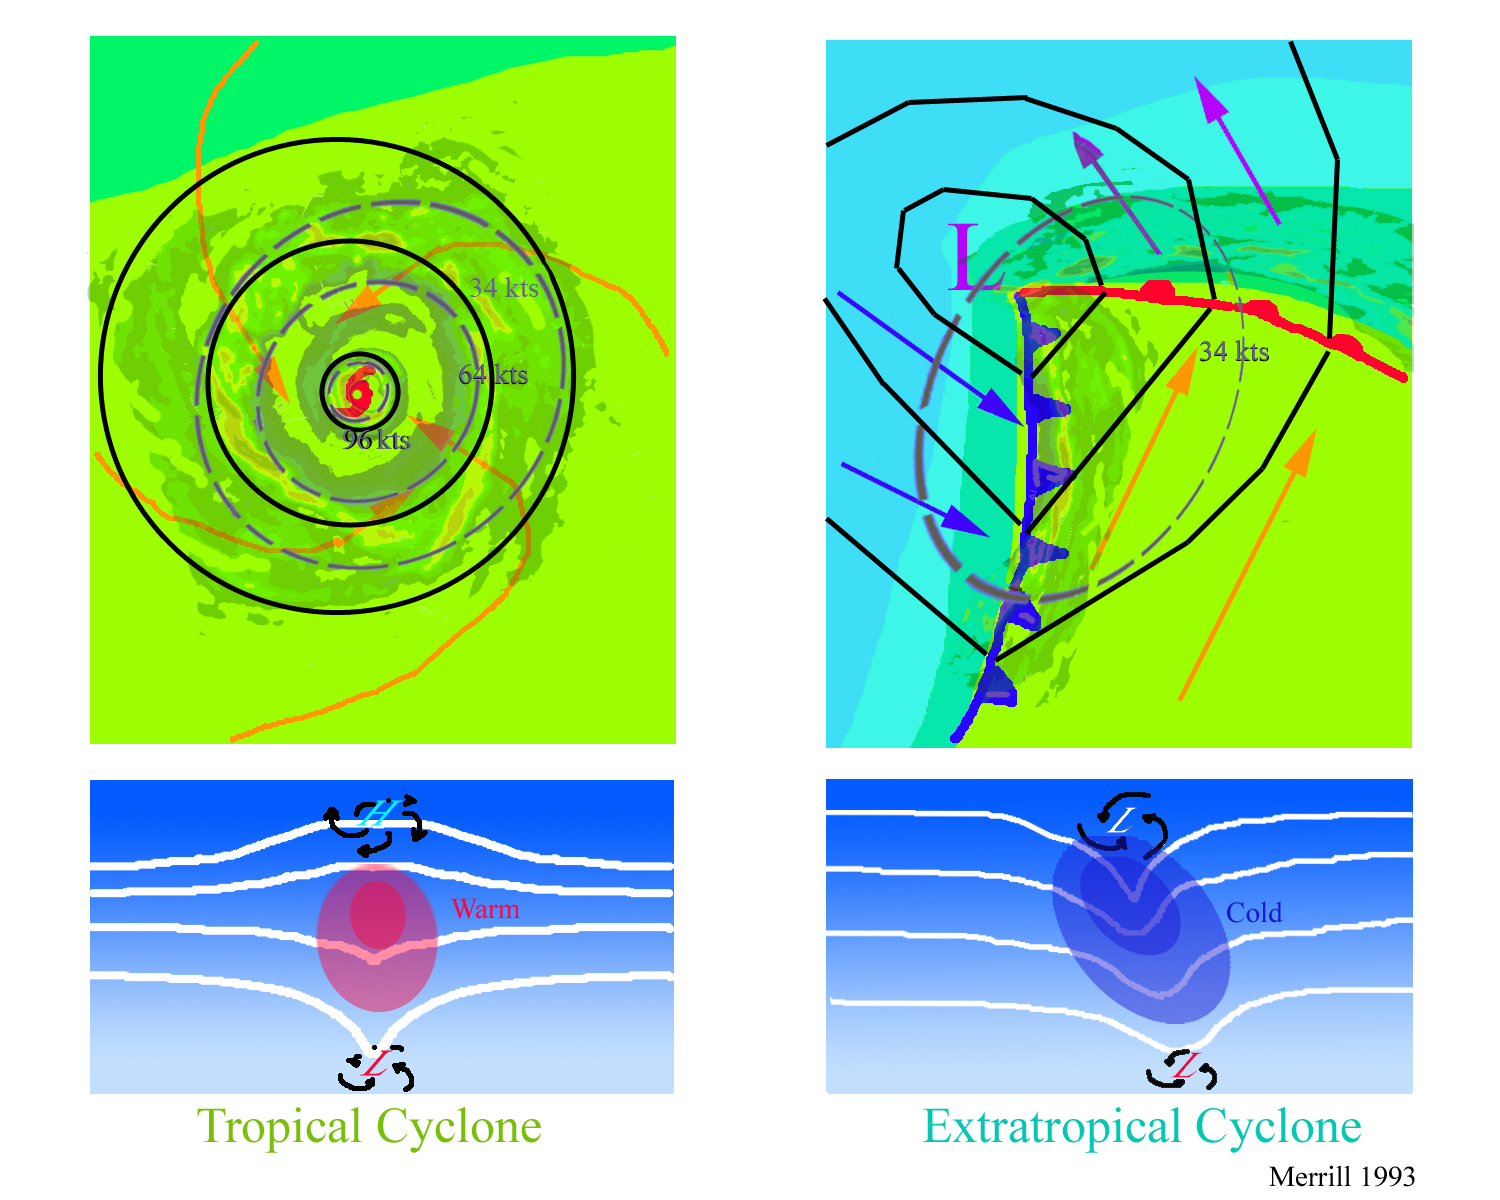
\includegraphics[width=22pc,angle=0]{trop-extra.jpg}
	\caption{Comparison of tropical cyclone and extra-tropical cyclones. The top schematics show horizontal maps of the surface temperature, pressure, and wind fields associated with a tropical cyclone (left) and an extratropical cyclone (right). Colours indicate temperature (blue 15C, blue green 20C, green 25C). Dashed lines indicate surface windspeeds : 34 kt=39 mph, 64 kt=74 mph, and 96 kt=110 mph. Solid lines are isobars. The bottom schematics show vertical maps of the pressure surfaces, temperature anomalies, and circulation at the surface and tropopause. \cite{NOAA}}\label{fig:trop-extra} %http://www.aoml.noaa.gov/hrd/tcfaq/A7.html
\end{figure}

Figure \ref{fig:trop-extra} shows the axisymmetric structure of a tropical cyclone and the frontal structure of an extra-tropical cyclone. The tropical cyclone has a warm core and an extra-tropical cyclone is cold core, with a slanted vertical profile. (Explain warm core vs cold core).

Extra-tropical cyclones are a dominant feature of the mid-latitudes, associated with strong winds, precipitation and temperature changes. An extra-tropical cyclone is a low pressure system that primarily gets its energy from a horizontal temperature gradient. This is in contrast to tropical cyclones, where there is little temperature contrast across them and they get their energy from the underlying ocean. Extra-tropical cyclones are moved by the jet stream and by other large-scale components of the global circulation \citep{stull}. They have frontal features, i.e. they are associated with cold fronts, warm fronts, and occluded fronts and in the northern hemisphere have winds counter clockwise, embedded in mid-latitude westerlies, travelling in an eastward direction. Like tropical cyclones, they transport heat and moisture from the Tropics towards the poles.

The variability of extra-tropical storm activity is due to both atmospheric and ocean conditions. These storm systems extend through the atmosphere, however, underlying conditions in the marine boundary layer (MBL) are important too. The MBL is the part of the atmosphere that lies over the ocean surface and is directly influenced by it.  Variations in the ocean surface therefore affect the cyclone, affecting ocean-atmosphere exchanges of heat, moisture and momentum. Major storm tracks are organised along or just downstream of the main oceanic frontal zones (Nakamura et al 2004).

%%%%%% Impact and importance of forecasting %%%%%%

Tropical cyclones are the most devastating natural hazards, affecting large populations in both the developed and developing world. Most of the damage occurs when tropical cyclones make landfall, and it is not only the destructive force of the strong winds, but also heavy precipitation and storm surge that cause widespread damage to communities.

Storm surges are responsible for much of the damage associated with landfalling tropical cyclones \citep{lin2012physically}. Storm surge is complicated, determined by the characteristics of the storms as well as shape and bathymetry of the coast, and the importance of the storm characteristics whilst over the open ocean and before landfall are also important. Rainfall distribution and intensity is complicated and depends on interactions on a variety of scales, with track, intensity, topography and environmental vertical shear all having an impact. Tropical storm wind fields change drastically when they make landfall, involving a complex interaction with the system and the underlying surface. The maximum damage of a tropical cyclone is not always at the point of landfall, but can be when it is further inland, for example when heavy rainstorms caused by interaction with mid-and lower-latitude systems once the storm is overland occur \citep{xiao2013analysis}. Although most damage occurs when tropical storms make landfall, they can also cause significant damage whilst at sea, mainly to the offshore industry.

%Loading on offshore structures is a complex function of not only characteristics of the wind field but also ocean characteristics including currents and waves \citep{done2014future}. Tropical-cyclone-wind resistant turbines have been deployed off the coast of China \citep{clark2014global}, to increase resilience to any future storms.

Such landfalling typhoons also have a significant economic impact, for example Super Typhoon Herb (1996) caused 73.26 billion yuans  (£8.31 billion) in direct economic losses and became the costliest landfalling tropical cyclone in China at the time \citep{zhang2009tropical}.
%In China, there is an upward trend in the economic cost of landfalling tropical cyclones, and this is principally caused by economic development \citep{zhang2009tropical}.

Damage from extra-tropical cyclones is also due to storm surge, strong winds, heavy precipitation and thunderstorms. The "Great Storm of 1987" struck the UK in October and had winds gusting at up to 100 mph with widespread devastation, 18 lives lost, around 15 million trees blown down and massive economic cost \citet{GreatStorm}. Tropical cyclones can become extra-tropical cyclones through a process called extra-tropical transition. Such a storm was ex-hurricane Sandy, which was one of the largest storms ever recorded in the Atlantic, with gale force winds extending 870 nautical miles in diameter \citet{blake2013tropical}. 
% https://www.metoffice.gov.uk/learning/learn-about-the-weather/weather-phenomena/case-studies/great-storm
% https://www.nhc.noaa.gov/data/tcr/AL182012_Sandy.pdf
%Lothar, Martin, clustering

The huge impacts that can be caused by both tropical and extra-tropical cyclones makes it vital to have good prediction skill of such phenomena across all time scales. Weather forecasting of such events has improved significantly over past decades, with increasing resolution and model complexity. The complex interactions between the atmosphere and ocean and the synoptic scale storm with global circulation requires accurate representation of processes within the model on different scales as well as interaction between the different model components.


\section{Summary}

Tropical and extra-tropical cyclones can cause significant damages and so their forecasting is vital. Tropical cyclones draw their energy from the heat in the underlying ocean, whereas extra-tropical cyclone feed off baroclinicity in the atmosphere. Both synoptic-scale phenomena are controlled by processes in the ocean as well as the atmosphere.

%Difference between Tropics and extra-Tropics, ie atmosphere-ocean forcing. Difference in storm systems, size frequency, variabolity, prediction and modelling, downstream effect and impact.


%%%%%%%%%%%%%%%%%%%%%%%%%%%%%%%%%%%%%%%%%%%%%%%%%%%%%%%%%%%%%%%%%%%%%%%%%%%%%

%http://www.air-worldwide.com/Press-Releases/AIR-Estimates-Insured-Losses-from-Super-Typhoon-Haiyan-at-Between--USD-300-Million-and-USD-700-Million/

% From zhang2009tropical: In an average year, landfalling tropical cyclones cause 472 deaths and 28.7 billion yuans (2006 RMB) in direct economic losses, accounting for 0.38% of the annual total gross domestic product (GDP) of China. As the deadliest landfalling tropical cyclone, Super Typhoon Fred killed 1,126 people in 1994, making it the deadliest year (1,815 deaths). The costliest landfalling tropical cyclone was Super Typhoon Herb, which caused 73.3 billion yuans (2006 RMB) in direct economic losses in 1996, making it the costliest year (107.9 billion yuans). The direct economic losses and casualties of a landfalling tropical cyclone tend to increase with the northward shift in landfall track.

%The atmosphere can maintain the TC or destroy it, principally through vertical wind shear.
%One hypothesized pathway by which vertical shear affects tropical cyclones is mid-level ventilation, or the flux of low-entropy air into the centre of the tropical cyclone \citep{McBride1995}. Tropical upper tropospheric trough (TUTT) cells from the mid-latitudes can weaken tropical cyclones by introduction of vertical wind shear, but also bring a cyclonic PV anomaly, which may contribute to intensification \citep{zeng2007environmental}.
%EXPLAIN
%Strong vertical wind shear prohibits rapid intensification and most likely results in the weakening of TCs \citep{zeng2007environmental}.
%and a threshold of 12.5 ms$^-1$ above which TCs cannot form in the WPAC has been suggested \citep{zehr1992tropical}-seems to be a thesis - check this ref
%e and Zehr 1991, Zehr 1992 - thesis?)
%check zeng paper
% McBride and Tang for ventilation

% Fast translation speed and strong vertical shear and detrimental to TC intensification \citep{zeng2007environmental} and

%WPSH is highly predictable and this can be used for tropical storm predictions \citep{wang2013subtropical}.

%Modes of variability - see Zhan 2012 review.
%Steering - Harr and Elsberry - straight, recurving, recurving north.
%IOD
%The intensity of a given storm depends on its surrounding environment.
%wang2013subtropical - Indian Ocean refs.

%Know about tropical waves - see Lu seasonal paper.

%IO importance - on MT?


%what kind of intensities? named?

%Conditions favourable to cyclogenesis are a baroclinic atmosphere (a region of large temperature change across a short horizontal distance near the surface), there is often an associated a strong jet stream running parallel at upper levels.
%what about mositure?
%cyclogenesis involves sea-level pressure decrease as the low pressure centre deepens, upward-motion increase, and vorticity increase.

%Baroclinic instability is due to a horizontal temperature gradients in a rotating environment. 

%What season? winter storms or summer storms? extratropical transition?

%extratropical ocean-atmosphere interaction dominated by atmosphere forcing the ocean, but with variability with oceanic processes more important to SST in the vicinity of WBCs (smirnow).

%baroclinic wave, steering level. Steered by large scale, much like TCs?

%Due to variations in the atmosphere and ocean - baroclinic atmosphere required for cyclogenesis (ref section). 

%Sheldon(The atmosphere above the Northern Hemisphere’s western boundary currents (the Gulf Stream and Kuroshio) are maximums in the winter atmospheric variability on a synoptic timescale of 2-6 days (Lau and Wallace, 1979; Blackmon, 1976; Hoskins and Valdes, 1990). These regions of synoptic variability are called the storm tracks and the variability is measuring the growth of extra-tropical cyclones that occur there (Dacre and Gray, 2009).)

%\cite{nakamura2004observed}
%As the surface air temperature over the open ocean is linked to SST underneath, maritime surface baroclinic zones tend to be anchored along oceanic fontal zones [NS04]. Though acting as thermal damping for the evolution of individual  eddies, heat exchange with the underlying ocean, on longer time scales, can act to restore atmospheric near-surface baroclinicity against the relaxing effect by atmospheric eddy heat transport, as evident in sharp meridional contrasts in upward turbulent heat fluxes observed climatologically across midlatitude frontal zones [Oberhuber, 1988]. Some observations are shown in section 2 to suggest that SST anomalies in a midlatitude frontal zone can likely play a more active role in the air–sea interaction than act to damp  tmospheric anomalies thermally Hoskins and Valdes (1990) mean diabatic heatin as a result of the warm ocean current restores the meridional atmostpheric temperature gradient and therfore baroclinciiy, that is vital to the storm tracks existence.

%nakamura et al 2008 \cite{nakamura2008importance}
%and booth et al 2010 - air-sea heat exchanges at oceanic fronts restore the baroclinicity of the atmosphere at low levels.
%shear instability not parametrised in current generation of GCMs.

%GCMs generally simulate the storm tracks well (d'Andrea et al 1998)as they are large-scale phenomenon of the atmospheric circulation. Also climate models can capture the structure of ETCs (cite{\catto2010can}).
%Atmosphere-ocean interactions are their strongest over WBCs, e.g Gulf Stream. Strong fluxes of heat and moisture anchor the storm tracks to the WBCs (Nakamura et al 2004). allows for recurrent develpoment of storm tracks - creates baroclinicity?

%Deep ascent over the Gulf Stream is a result of extreme events, i.e. extra-tropical storms \citep{minobe2008influence}(check this)
%The storms occur in these locations as the strong oceanic fronts help maintain the surface baroclinicity required to produce them (Nakamura and Shimpo, 2004 Nakamura et al., 2008; Sampe et al., 2010).  (sheldon thesis).
%SHELDON THESIS:
%The Gulf Stream is the western boundary current for which the most links to deep convection have been found. %The deep ascent over the Gulf Stream found by Minobe et al. (2008) is a result of extreme events that skew the mean to ascent, and their results do not represent an average day in that region. The ascent above the Gulf Stream being a product of extreme events is consistent with the region also being the centre of action for winter synoptic systems in the Northern Hemisphere (Hoskins and Valdes, 1990).


